\section{Результат выполнения программы}

Как уже было сказано в предыдущих разделах пояснительной записки,
данная реализация интерпретатора языка Бейсик способна выявить
все лексические, синтаксические и семантические ошибки в 
исходном коде программы на этапе ее разбора.

В случае возникновения ошибок разбора программы происходит
срабатывание исключительной ситуации определенного типа.

Для того, чтобы пользователь мог с легкостью сопоставить
полученную от интерпретатора ошибку с содержимым своего
исходного кода и исправить ее перед следующим запуском,
необходимо, чтобы получаемые им ошибки были интерактивными.

В разделе \ref{class-description} содержится описание класса \emph{Monitor}, 
который перехватывает возникающие исключения и 
преобразует их в информативное сообщение с указанием
на ошибку. 

На рисунках (\ref{error1} - \ref{error5}), приведенных ниже,
можно увидеть результат выполнения программы интерпретатора
при обработке исходных программ, содержащих некоторые
ошибки.

\begin{figure}[H]
    \centering
    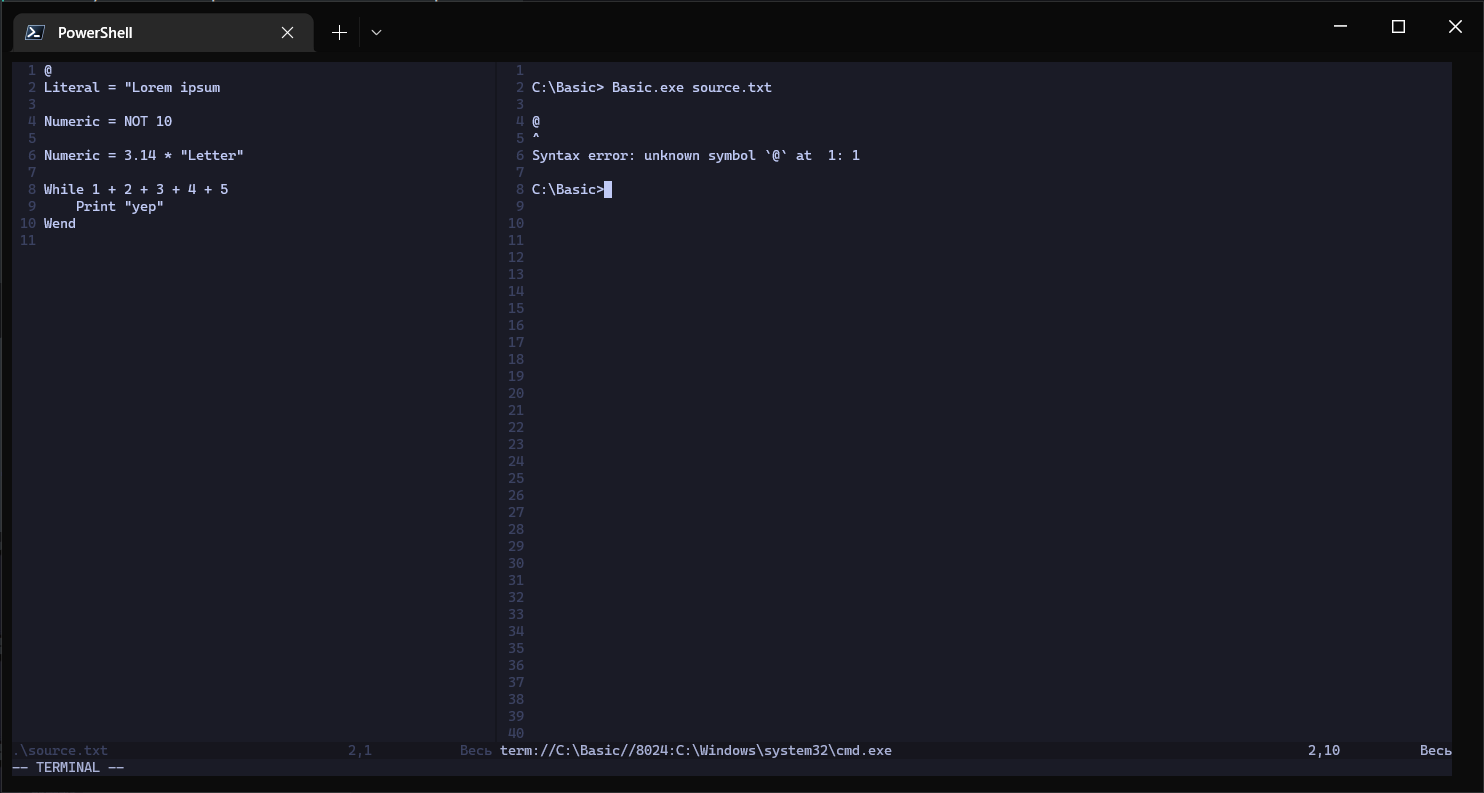
\includegraphics[scale=0.42]{image1.png}
    \caption{Синтаксическая ошибка 'неизвестный символ'}
    \label{error1}
\end{figure}

\begin{figure}[H]
    \centering
    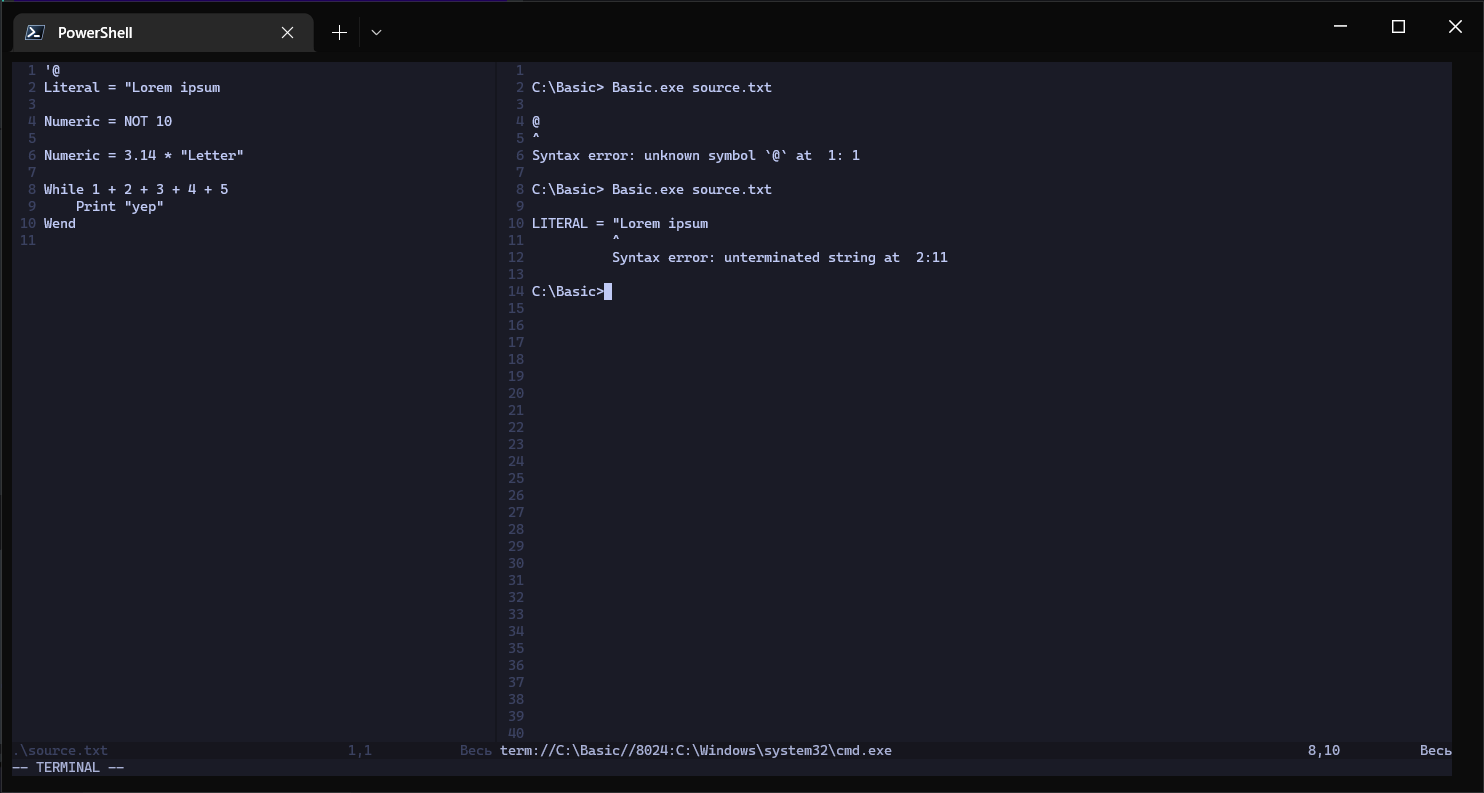
\includegraphics[scale=0.42]{image2.png}
    \caption{Синтаксическая ошибка 'незаконченная строка'}
    \label{error2}
\end{figure}

\begin{figure}[H]
    \centering
    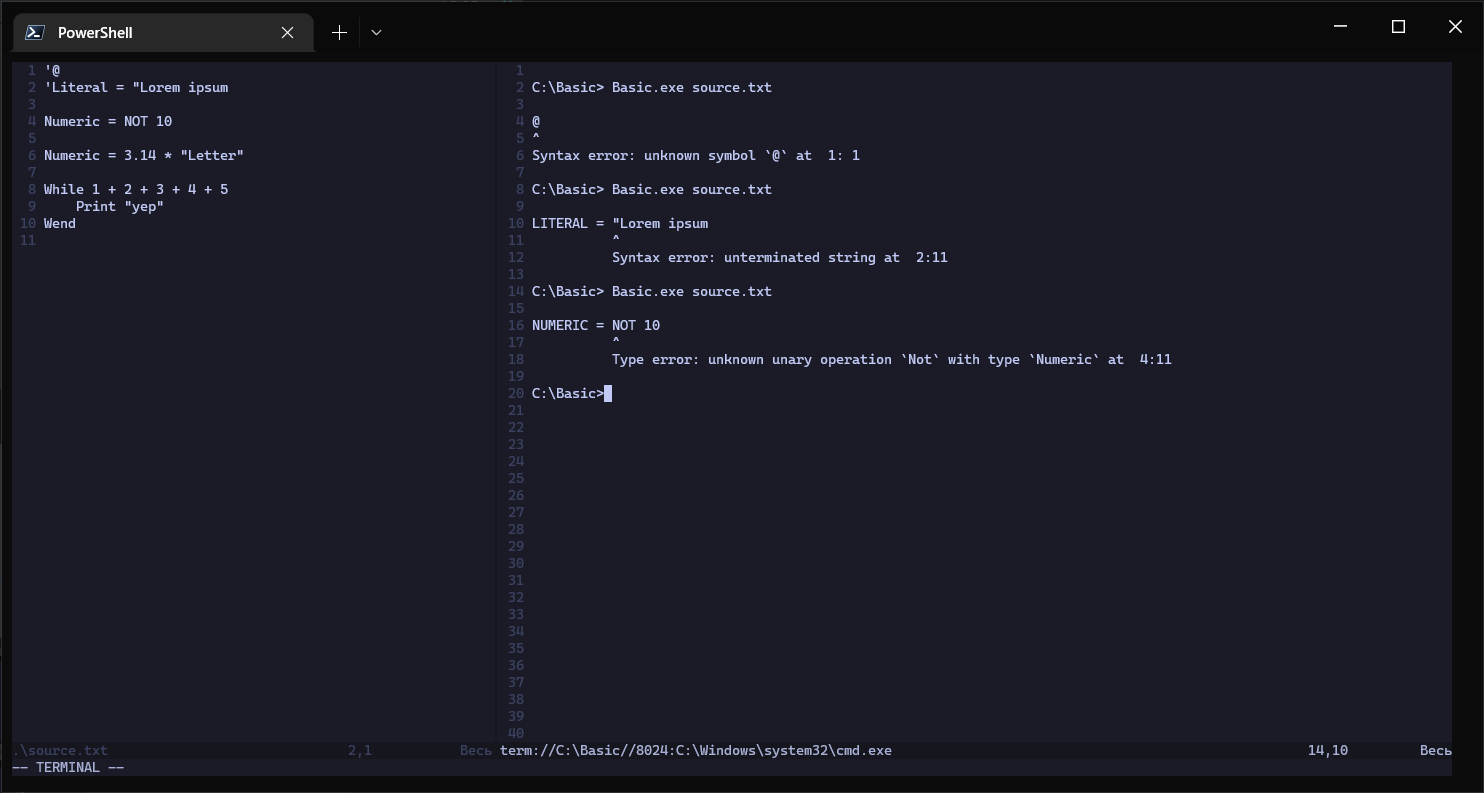
\includegraphics[scale=0.42]{image3.png}
    \caption{Синтаксическая ошибка 'неизвестная унарная операция'}
    \label{error3}
\end{figure}

\begin{figure}[H]
    \centering
    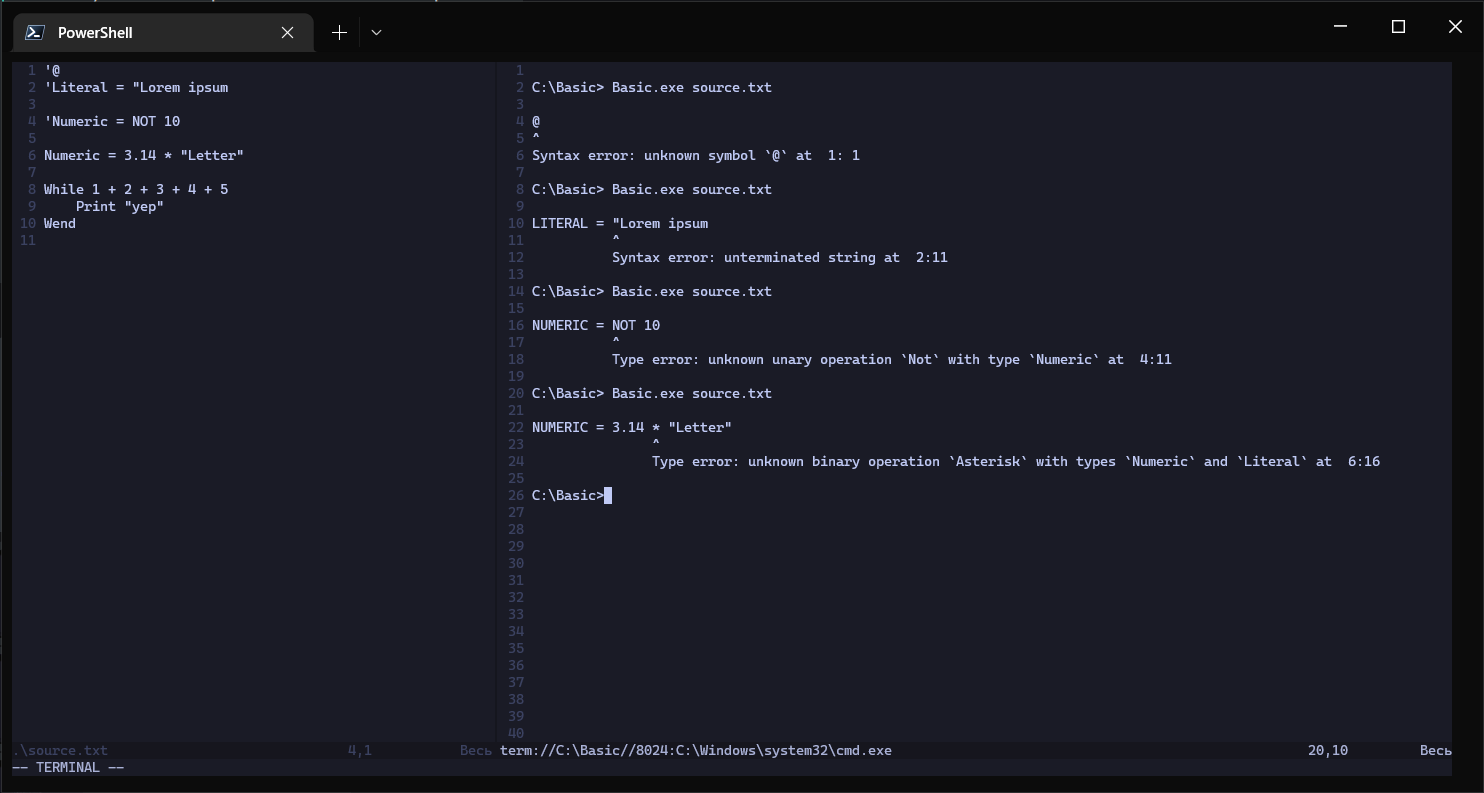
\includegraphics[scale=0.42]{image4.png}
    \caption{Синтаксическая ошибка 'неизвестная бинарная операция'}
    \label{error4}
\end{figure}

\begin{figure}[H]
    \centering
    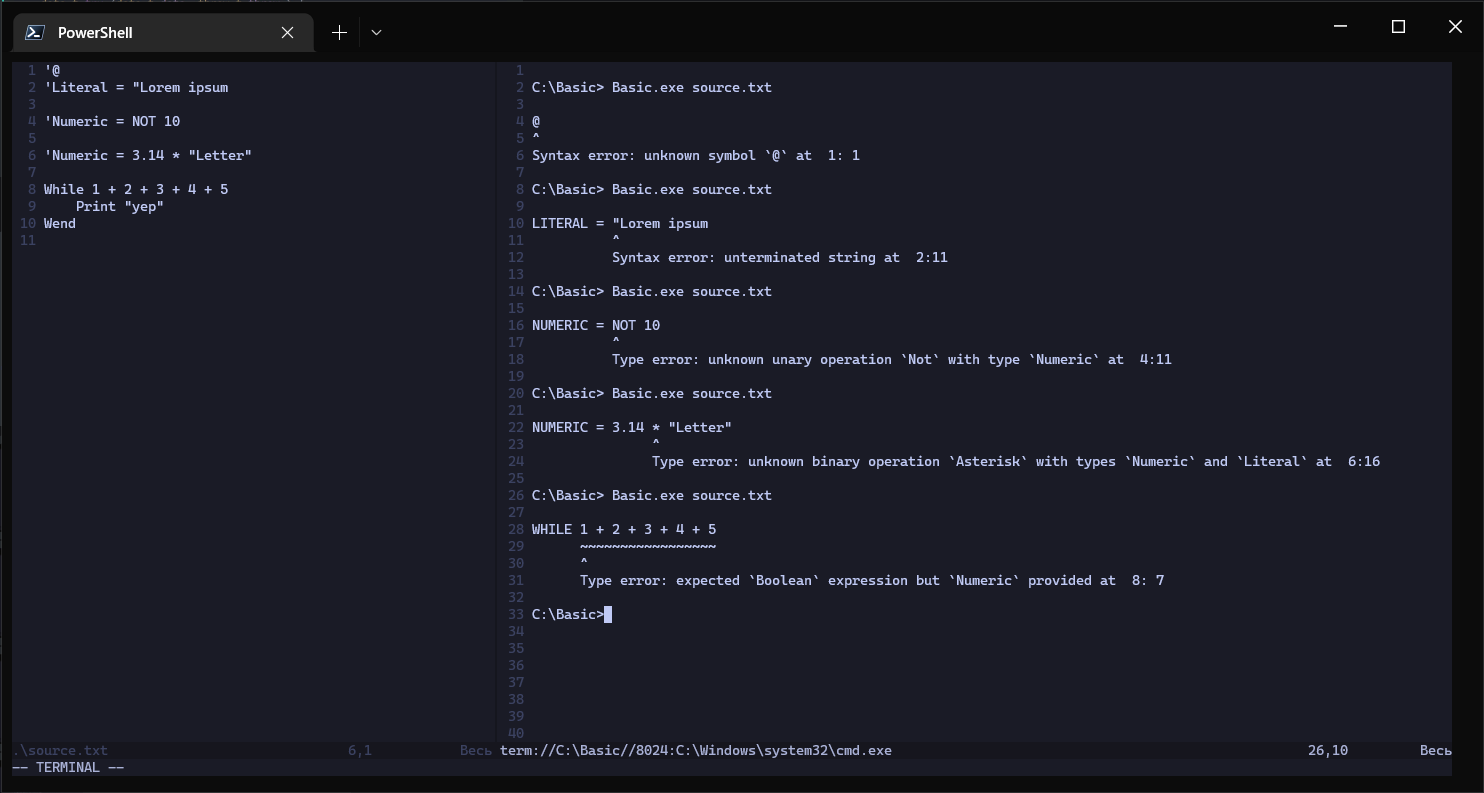
\includegraphics[scale=0.42]{image5.png}
    \caption{Синтаксическая ошибка 'неверный тип выражения'}
    \label{error5}
\end{figure}

\pagebreak

На рисунке \ref{guessing} изображен результат выполнения
программы, реализующей простую математическую игру <<Угадай число>>.

\begin{figure}[hb]
    \centering
    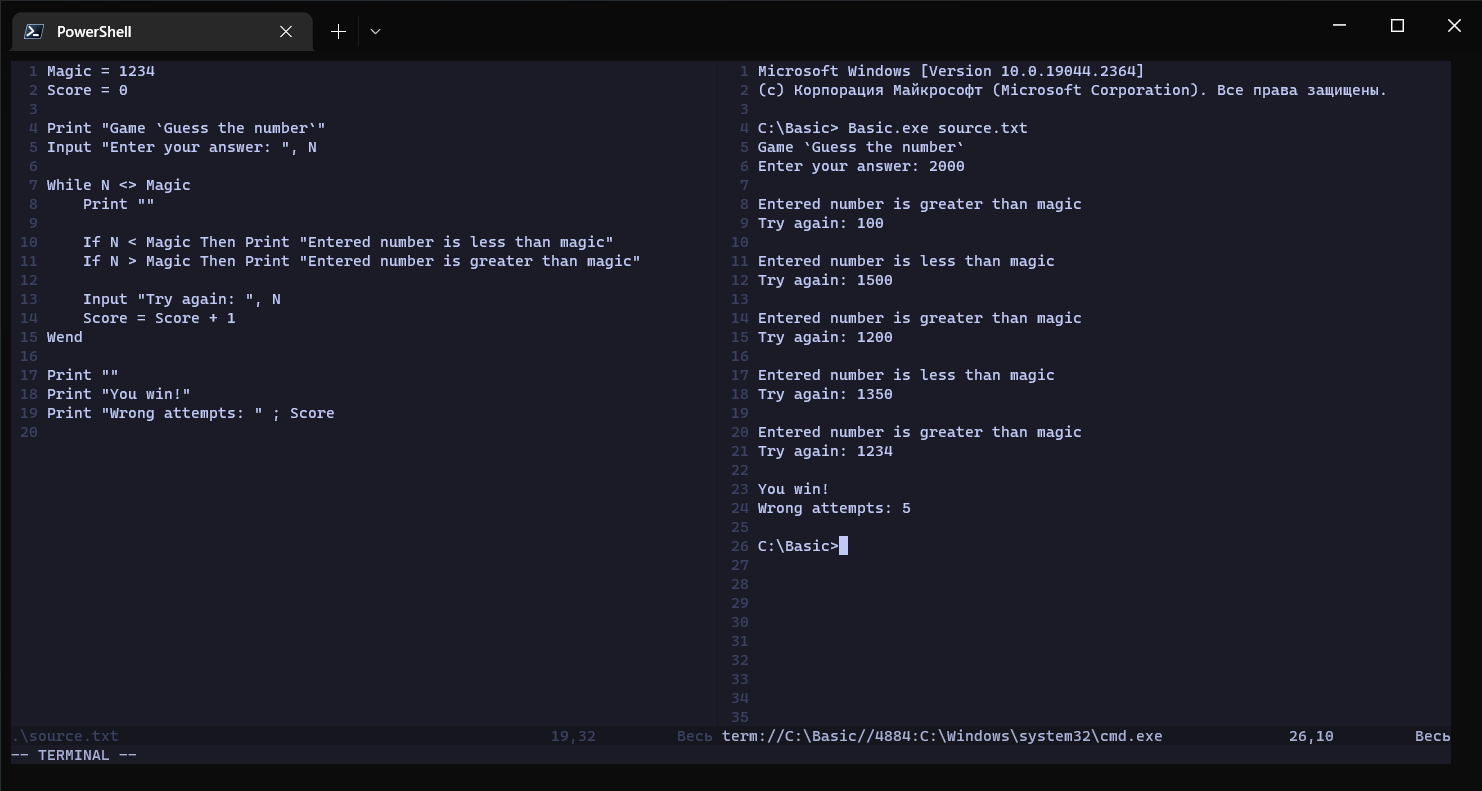
\includegraphics[scale=0.42]{image6.png}
    \caption{Результат успешного выполнения программы}
    \label{guessing}
\end{figure}